\documentclass[a5paper,titlepage,10pt,openany]{scrbook}
\usepackage[a5paper,backref]{hyperref}
\usepackage[papersize={148.5mm,215mm},twoside,bindingoffset=0.5cm,hmargin={2cm,2cm},
				vmargin={2cm,2cm},footskip=1.1cm,driver=dvipdfm]{geometry}
\usepackage{palatino}
\usepackage{pstricks}
\usepackage{graphicx}
\usepackage[bahasa]{babel} 
%\usepackage[pdftex]{dropping}
\usepackage{lettrine}
\usepackage{pifont}
\usepackage{enumitem}
\usepackage{wrapfig}
\usepackage{indentfirst}
\usepackage{parcolumns}
\usepackage[titles]{tocloft}
\usepackage{longtable}
%\usepackage[raggedright]{titlesec}
%\usepackage{titletoc}


\renewcommand{\cftchapfont}{%
  \fontsize{9}{8}\selectfont
}

\makeatletter
\renewcommand{\@pnumwidth}{1em} 
\renewcommand{\@tocrmarg}{1em}
\makeatother

\author{Lingkungan St. Petrus Maguwo}
\title{Warta Iman}
\setlength{\parindent}{1cm}
\psset{unit=1mm}

\makeatletter
\renewcommand{\@makeschapterhead}[1]{%
  {\parindent \z@ \centering \normalfont
    \interlinepenalty\@M \Large \bfseries #1\par\nobreak \vskip 20\p@ }}
\renewcommand{\section}{\@startsection {section}{1}{\z@}%
                                   {-3.5ex \@plus -1ex \@minus -.2ex}%
                                   {2.3ex \@plus.2ex}%
%                                   {\normalfont\normalsize\bfseries\centering}}
                                   {\normalfont\normalsize\bfseries}}
\renewcommand\subsection{\@startsection{subsection}{2}{\z@}%
                                     {-3.25ex\@plus -1ex \@minus -.2ex}%
                                     {1.5ex \@plus .2ex}%
                                     {\normalfont\normalsize\bfseries}}
\renewcommand\subsubsection{\@startsection{subsubsection}{3}{\parindent}%
                                    {3.25ex \@plus1ex \@minus.2ex}%
                                    {-1em}%
                                    {\normalfont\normalsize\bfseries}}

\makeatother

\makeatletter  % Allow the use of @ in command names
\long\def\@makecaption#1#2{%
  \vskip\abovecaptionskip
  \sbox\@tempboxa{{#1#2}}%
  \ifdim \wd\@tempboxa >\hsize
    {#1#2\par}
  \else
    \hbox to\hsize{\hfil\box\@tempboxa\hfil}%
  \fi
  \vskip\belowcaptionskip}
\makeatother   % Cancel the effect of \makeatletter

\newcommand{\chap}[1]{%
    \chapter*{#1}
	\addcontentsline{toc}{chapter}{#1}
    }

\newcommand{\sumber}[1]{%    
	\begin{flushright}
	{\emph{#1}}
	\end{flushright}
}
\newcommand{\qti}[1]{%    
	\begin{quote}
	{\emph{#1}}
	\end{quote}
}

\hyphenation{sa-u-da-ra-ku}
\hyphenation{ke-ri-ngat}
\hyphenation{je-ri-tan}
\hyphenation{hu-bung-an}
\hyphenation{me-nya-dari}
\hyphenation{Eng-kau}
\hyphenation{ke-sa-lah-an}
\hyphenation{ba-gai-ma-na}
\hyphenation{Tu-han}
\hyphenation{di-per-ca-ya-kan}
\hyphenation{men-ja-uh-kan}
\hyphenation{bu-kan-lah}
\hyphenation{per-sa-tu-kan-lah}
\hyphenation{ma-khluk}
\hyphenation{Sem-buh-kan-lah}
\hyphenation{ja-lan}
\hyphenation{mem-bu-tuh-kan}
\hyphenation{be-ri-kan-lah}
\hyphenation{me-ra-sa-kan}
\hyphenation{te-man-ilah}
\hyphenation{mem-bi-ngung-kan}
\hyphenation{di-ka-gum-i}
\hyphenation{ta-ngis-an-Mu}
\hyphenation{mi-lik-ilah}

\renewcommand{\figurename}{~}
\renewcommand\thefigure{~}

\setlength{\itemsep}{0cm}

\begin{document}
\setlength{\parindent}{1cm}
\thispagestyle{empty}
\thispagestyle{empty}
\newcommand{\edisi}[1]{%
\DeclareFixedFont{\PT}{T1}{ppl}{b}{}{0.7in}
\DeclareFixedFont{\PTit}{T1}{ppl}{b}{it}{0.7in}
\DeclareFixedFont{\PTsmall}{T1}{ppl}{b}{it}{0.25in}
\DeclareFixedFont{\PTsmaller}{T1}{ppl}{b}{it}{0.175in}
\DeclareFixedFont{\PTsmallest}{T1}{ppl}{b}{it}{0.15in}

\begin{pspicture}(14cm,2cm)
\rput[rb](10.35cm,3cm){\PTsmallest {#1}}
\rput[lb](-2cm,1.5cm){\PT {WARTA IMAN}}
\rput[lb](0cm,0.5cm){\PTsmall {Lingkungan St. Petrus Maguwo}}
\end{pspicture}%
}

\newcounter{kgkcounter}[chapter]
\renewcommand{\thekgkcounter}{\arabic{kgkcounter}. }
\newcommand{\kgk}[1]{\refstepcounter{kgkcounter}\textbf{\flushleft \textbf{\thekgkcounter #1}}\\}

\newcommand{\kutipan}[1]{%
\noindent{\framebox{\parbox{10cm}{\centering\emph{#1}}}}}

\edisi{November 2011}

%\vspace{1cm}

\begin{center}
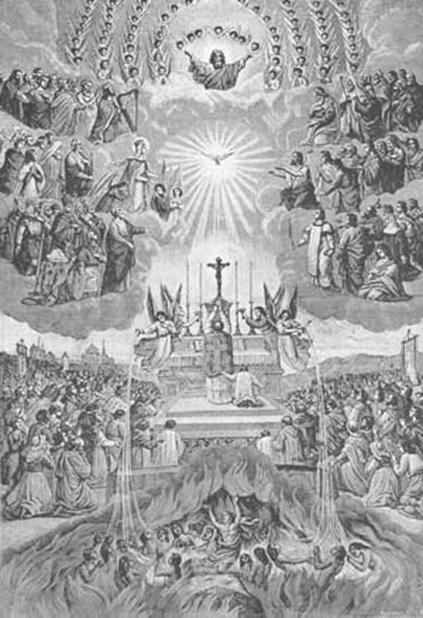
\includegraphics[scale=0.85]{gambar/purgatory2.jpg}
\end{center}

%\vspace{1cm}

\begin{center}
{\PTsmaller {Kasih, kerendahan hati, dan menurut pada kehendak Allah }}
\end{center}


\newpage

\begin{parcolumns}[colwidths={1=0.7\textwidth},distance=0.4cm]{2}
\colchunk{
\parbox[t]{0.7\textwidth}{
\newpage

\chapter*{Dari Redaksi}
\footnotesize
\indent{Berkah Dalem,}
Bulan Maret sudah memasuki masa Prapaskah. Tidak ada salahnya jika kita mengambil tema \textit{Prapaskah} untuk edisi kali ini. Mungkin kita masih bertanya-tanya kenapa setiap masa prapaskah kita berpuasa dan berpantang. Bagian awal WI edisi kali mencoba menjawab pertanyaan tersebut.

\bigskip
Menjelang prapaskah kita sudah mendengar pembacaan pesan Bapa Uskup dalam menyongsong masa prapaskah. Dalam edisi ini Anda dapat menyimak pesan dari Bapa Paus Benediktus dalam rangka menyongsong Prapaskah 2012.

\bigskip
Masa prapaskah diawali dengan hari Rabu Abu. Kenapa Rabu dan kenapa abu? Juga kenapa digunakan daun palm bukan yang lain? Jawabannya dapat Anda simak dalam edisi kali ini. 
 
\bigskip
Renungan tentang 4 prinsip hidup dan ketika garam kehilangan asinnya melengkapi edisi kali ini. Kutipan Kompendium Gereja Katolik masih berlanjut sampai pada nomor 30 -- 33.

\bigskip

Warta lingkungan kali ini tidak memuat pasangan yang berulangtahun, karena data yang ada redaksi tidak ditemukan warga St. Petrus yang berulangtahun perkawinan bulan Maret. Redaksi tetap berharap partisipasi umat untuk meramaikan rubrik ini dengan mengirim sms berupa saran, kritik, pertanyaan, atau sekedar \textit{uneg-uneg}, dengan harapan terjalin komunikasi antar umat dan juga pengurus. Tema bulan April adalah Paskah sedang bulan Mei adalah Liturgi. Sekali lagi ditunggu partisipasi seluruh umat.
\normalsize

\begin{center}***\end{center} 

\vfill

\noindent{\framebox{\parbox{10cm}{\small
Warta Iman\\
Media komunikasi dan informasi umat lingkungan St. Petrus\\
Alamat Redaksi: Lingkungan St. Petrus Maguwo\\
E-mail: stpetrusmgw@gmail.com
}}}
\normalsize

}
}
\colchunk{
\setlength{\parindent}{0cm}
\parbox[t]{0.25\textwidth}{
\tableofcontents}
\setlength{\parindent}{1cm}
}
\colplacechunks
\end{parcolumns}

\setlength{\parindent}{1cm}

\chap{Baptisan dan Hidup Baru}

Banyak orang Protestan mengatakan dan percaya bahwa baptis hanya sebuah simbol. Dalam Gereja Katolik baptisan tidak hanya sebagai simbol tetapi adalah sebuah sakramen. Baptisan (menurut Gereja Katolik) membuat kita lahir baru. Dasar kitab suci dari ajaran tentang baptis ini cukup banyak antara lain:

Yohanes 3:5 "Aku berkata kepadamu, sesungguhnya jika seorang tidak dilahirkan dari air dan Roh, ia tidak dapat masuk ke dalam Kerajaan Allah" pada ayat ini Yesus menekankan pentingnya baptis sebagai jalan untuk masuk dalam Kerajaan Allah.

Dalam Kis 2:38 St. Petrus mengatakan "Bertobatlah dan hendaklah kamu masing-masing memberi dirimu dibaptis dalam nama Yesus Kristus untuk pengampunan dosamu, maka kamu akan menerima karunia Roh Kudus." St. Petrus menekankan perlunya baptis untuk pengampunan dosa dan syarat untuk menerima karunia Roh Kudus.

St. Paulus dalam Titus 3:5 "Pada waktu itu Dia telah menyelamatkan kita, bukan karena perbuatan baik yang telah kita lakukan, tetapi karena rahmat-Nya oleh permandian kelahiran kembali dan oleh pembaharuan yang dikerjakan oleh Roh Kudus" lalu dalam Kis 22:16 "Dan sekarang, mengapa engkau masih ragu-ragu? Bangunlah, berilah dirimu dibaptis dan dosa-dosamu disucikan sambil berseru kepada nama Tuhan!"

Dari beberapa ayat diatas jelaslah bahwa Sakramen baptis bukan hanya sebuah lambang atau simbol (jikalau itu simbol untuk apa Para Rasul menekankan perlunya baptis?) tetapi baptisan memang membuat kita lahir baru, karena baptisan itu berhubungan erat sekali dengan Roh Kudus yang membuat kita lahir baru. Bila kita perhatikan Yohanes 3:5 "Aku berkata kepadamu, sesungguhnya jika seorang tidak dilahirkan dari air dan Roh, ia tidak dapat masuk ke dalam Kerajaan Allah" kata "air dan Roh" (Baptisan dan Roh Kudus) memiliki suatu hubungan erat yang tidak dapat dipisahkan. Hubungan yang erat antara baptisan dan Roh Kudus yang tak terpisahkan inilah yang membuat kita memperoleh hidup baru pada saat kita dibaptis. Karena hubungan yang erat antara Roh Kudus dan baptisan sehingga ketika Paulus berbicara mengenai baptisan ia tidak menyebut Roh Kudus "Atau tidak tahukah kamu, bahwa kita semua yang telah dibaptis dalam Kristus, telah dibaptis dalam kematian-Nya? Dengan demikian kita telah dikuburkan bersama-sama dengan Dia oleh baptisan dalam kematian, supaya, sama seperti Kristus telah dibangkitkan dari antara orang mati oleh kemuliaan Bapa, demikian juga kita akan hidup dalam hidup yang baru." (Roma 6:3-4).

Baptisan bukan perbuatan manusiawi belaka tetapi baptis adalah tanda dan sarana Rahmat Allah (yaitu kelahiran/hidup baru) dimana Allah berkarya melalui para pelayan (Imam, Diakon, dll) yang membaptis. Jadi baptisan adalah karya Allah sendiri yang mencurahkan Roh Kudus-Nya. Baptisan tidak dapat dibedakan/ dipisahkan dari Iman kepada Yesus dan dari Pencurahan Roh Kudus. Baptisan merupakan perwujudan iman seseorang kepada Yesus dan Iman itu berhubungan dengan pencurahan Roh Kudus lihatlah pada 1 Kor 12:3 "Karena itu aku mau meyakinkan kamu, bahwa tidak ada seorangpun yang berkata-kata oleh Roh Allah, dapat berkata: "Terkutuklah Yesus!" dan tidak ada seorangpun, yang dapat mengaku: "Yesus adalah Tuhan", selain oleh Roh Kudus."

Dari uraian diatas jelaslah bahwa baptis bukan hanya sebuah simbol tetapi benar-benar membuat kita lahir baru karena peranan dari Roh Kudus yang membuat kita lahir baru didalam pembaptisan. Oleh karena hal itulah St. Petrus menegaskan perlunya baptisan bagi keselamatan "Juga kamu sekarang diselamatkan oleh kiasannya (kiasannya=air bah {lihat ayat sebelumnya untuk lebih jelas}), yaitu baptisan--maksudnya bukan untuk membersihkan kenajisan jasmani, melainkan untuk memohonkan hati nurani yang baik kepada Allah--oleh kebangkitan Yesus Kristus" (1 Pet 3:21)

\section*{Baptis cara Selam}
Setelah berbicara banyak mengenai Hakekat baptis yang membuat kita lahir baru, Ada baiknya kita membahas mengenai masalah baptis selam. Baptis selam dalam gereja Pantekosta  dimutlakkan dan mereka terkadang (tidak semuanya) mengatakan baptisan selain cara selam tidak sah.

secara umum terkadang mereka mengajukan bukti dari Matius 3:16 "Yesus segera keluar dari air" kata "keluar dari air" menurut mereka berarti Yesus sebelumnya berada didalam air. Menurut kami kata "keluar dari air" tidak menunjukkan berapa banyak bagian tubuh yang terendam (yang menarik bahwa lukisan Kristen kuno tentang  pembaptisan Yesus pada Katakombe, dll pada jaman yang dekat dengan jaman para rasul digambarkan bahwa Yesus masuk ke air hanya sebatas lutut). 

Yang agak Rumit disini adalah pembahasan dari kata Babtizo (kata Yunani untuk membaptis) yang menurut mereka berarti "menenggelamkan sesuatu dalam air". Sebenarnya kata Babtizo memiliki beberapa arti yaitu "menenggelamkan" dan arti yang lain "mencelupkan". Ada hal yang menarik bahwa Lukas 11:38 "Orang Farisi itu melihat hal itu dan ia heran, karena Yesus tidak mencuci tangan-Nya sebelum makan" kata "Mencuci" dalam Lukas 11:38 dalam bahasa Yunani babtizo tetapi dalam hal ini tentu bukan kata menenggelamkan, tetapi mungkin hanya mencelupkan (dalam tradisi yahudi ada tempayan yang digunakan untuk pembasuhan sebelum besantap) tetapi rasanya tidak etis dan tidak higienis jika seseorang mencelupkan tangannya (yang kotor) kedalam tempayan itu (sementara tempayan itu digunakan untuk pembasuhan tidak hanya untuk satu orang) tentunya orang akan mengambil gayung dan mengambil air dari tempayan itu lalu mengucurkannya ke tangan. Jadi jelaslah penggunaan kata "babtizo" sangat fleksibel tidak hanya menenggelamkan, oleh karena itu tradisi baptis Kristen sangat fleksibel (tidak hanya dengan diselam saja) berikut kesaksian dari Dokumen 12 Rasul (berasal dari abad II M) mengatakan bahwa jika tidak ada air yang cukup untuk membaptis maka pembaptisan dengan pengucuran airpun adalah sah. Hal itu juga ditegaskan dalam dokumen Didache (sekitar tahun 100 Masehi) yang berisi hal yang sama dan juga pernyataan St. Agustinus, sekedar pengetahuan Bahwa gereja Protestan yang termasuk aliran utama (Lutheran, Calvinis) menggunakan cara baptis mirip seperti Katolik. Kita tahu kitab suci tidak memberikan petunjuk yang jelas dengan cara apakah Para Rasul membaptis (apakah dengan cara selam, dibasuh, atau dengan cara lain) tetapi kesaksian Yustinus Martir bahwa pembaptisan dilakukan dengan cara "masuk ke air" dan menurut banyak sejarah Gereja, pembaptisan dilakukan dengan cara menenggelamkan orang dan ini merupakan cara baptis pada Gereja perdana yang akhirnya berevolusi menjadi Ritus yang lebih sederhana (untuk lebih jelasnya lihat: Sakramen baptis dan sejarah Perubahan Ritusnya). Cara (Ritus) apapun yang digunakan untuk pembaptisan tetap tidak mengubah hakekat sakramen baptis, bahkan menurut informasi di beberapa Gereja Katolik di Amerika terdapat "kolam" untuk membaptis. 

\section*{Keselamatan tanpa baptis?}
Dalam Dokumen Konsili Vatikan II Lumen Gentium No 16 dikatakan bahwa "Mereka yang tanpa bersalah tidak mengenal Injil Kristus serta Gereja-Nya, tetapi dengan tulus hati mencari Allah, dan berkat pengaruh rahmat berusaha melaksanakan kehendak-Nya yang mereka kenal melalui suara hati dengan perbuatan nyata, dapat memperoleh keselamatan kekal". Sekilas ajaran itu bertentangan dengan 1 Tim 2:5 "Karena Allah itu esa dan esa pula Dia yang menjadi pengantara antara Allah dan manusia, yaitu manusia Kristus Yesus" ajaran Konsili Vatikan II menegaskan bahwa mereka "yang tanpa bersalah tidak mengenal Injil Kristus" bisa selamat didasarkan karena Yesus menjadi tebusan bagi semua orang (lihat Mat 20:28; Mrk 10:45; 1Tim 2:6). Ajaran Konsili Vatikan II juga tidak bertentangan dengan Mrk 16:15 dan Yoh 3:18 karena menurut pendapat kami (yang bisa saja salah) Mrk 16:15 dan Yoh 3:18 tidak perlu ditafsirkan secara harafiah dalam arti yang ketat kedua  ayat itu menekankan tentang perlunya iman dan baptisan agar orang dapat selamat, namun bagi "yang tanpa bersalah tidak mengenal Injil Kristus" masakah mereka juga harus dihukum? Ajaran Konsili Vatikan II ini tidak mengakui bahwa semua agama itu sama, Gereja merasa perlu untuk mewartakan Injil dan kita wajib memperkenalkan Kristus yang adalah jalan kebenaran dan Kehidupan dan Gereja sendiri memiliki kepenuhan sarana-sarana keselamatan (lihat Redemptoris Missio 55, Ensiklik Evangelii Nuntiandi, dokumen Konsili Vatikan II Digitatis Humanae 14, Ad Gentes 6 dan 7, dll) oleh karena itulah Gereja tidak pernah melupakan Perutusan agung yang diberikan Yesus "Karena itu pergilah, jadikanlah semua bangsa murid-Ku dan baptislah mereka dalam nama Bapa dan Anak dan Roh Kudus, dan ajarlah mereka melakukan segala sesuatu yang telah Kuperintahkan kepadamu. Dan ketahuilah, Aku menyertai kamu senantiasa sampai kepada akhir zaman." (M at 28:19-20) dengan tujuan memperkenalkan Kristus yang adalah jalan yang pasti dan singkat menuju Rumah Bapa.

\sumber{Thomas Rudy http://www.imankatolik.or.id}
\chap{Sakramen Pembaptisan dan Sejarah Perubahan Ritusnya}

    Seperti sebuah karya seni yang telah diperbaiki, difernis sampai beberapa kali dan kadang kala sedikit disalahgunakan, ritus Sakramen Pembaptisan dalam Gereja Kristen juga telah mengalami perubahan selama berabad-abad dengan alasan dan latar belakang tertentu. Namun biarpun demikian, perubahan ritus itu tetap tidak mengubah hakekat Pembaptisan sebagai Sakramen tanda kelahiran baru seseorang ke dalam Kerajaan Allah di dalam Yesus Kristus. Tapi dewasa ini Gereja dihimbau untuk kembali ke ritus pembaptisan yang dipraktekkan oleh Gereja Kristen pada abad-abad pertama yaitu pembaptisan dengan dengan "mencelupkan" seorang catechumen ke dalam kolam air. Karena ritus pembaptisan seperti ini dirasa lebih efektif mengungkapkan peristiwa "kelahiran baru" seseorang ke dalam Karajaan Allah yang dimasukinya melalui Sakramen Permandian. Tapi demi alasan praktis, Gereja tetap diijinkan untuk memakai ritus pembaptisan sederhana dengan "menuangkan sedikit air pada kepala". Untuk lebih mamahami hal ini, mari kita kembali menengok sejarah Gereja seputar ritus sakramen permandian.

    ***

    Dalam bab pertama Injil Markus, seperti telah diramalkan Nabi Yesaya, Yohanes Pembaptis tampil di padang gurung sambil memaklumkan sebuah "pembaptisan pertobatan" demi pengampunan atas dosa. Orang banyak berkerumun mendengar kothbah Yohanes Pembaptis yang berkobar-kobar. Mereka berbondong-bon-dong ke Sungai Yordan dan memberi diri mereka untuk disucikan (Kata pembaptisan sendiri berasal dari kata Yunani "bapizo" yang berarti "membasuh atau mencelupkan atau menenggelamkan").

    Markus menceriterakan bahwa Yesus juga kemdian datang kepada Yohanes dan dibaptis. Ketika Ia keluar dari air, Ia melihat surga terbuka dan Roh Kudus dalam rupa seekor burung merpati turun ke atasNya. Dan Ia mendengar suara dari atas yang mengatakan:"Engkaulah PuteraKu yang terkasih; kepadamu aku berkenan."

    Penginjil Markus kemudian melanjutkan ceriteranya dengan mengatakan bahwa segera setelah peristiwa permandian di Sungai Yordan, Yesus dibawa Roh Allah ke padang gurun and tinggal di sana untuk berdoa dan berpuasa 40 hari lamanya, sambil digodai iblis. Setelah berdoa dan berpuasa, Yesus mulai menjalankan perutusanNya di depan umum.

    Lima belas bab kemudian, pada bagian akhir dari Injilnya, Penginjil Markus kembali mencatat kata-kata terakhir Yesus kepada kesebelas rasul (dikurangi Yudas Iskariot yang telah mengkianati Yesus): "Pergilah ke seluruh bumi dan wartakanlah Injil \dots ~Barangsiapa percaya dan dibaptis akan diselamatkan."

    Kalau kita meneliti Kitab Suci Perjanjian Baru (PB) maka kita akan menemukan kenyataan bahwa Kitab Suci PB tidak menceriterakan "bagaimana para Rasul membaptis". Tapi ahli sejarah Gereja berpendapat bahwa kemungkinan besar seorang calon permandian berdiri di air sungai atau di sebuah kolam umum, dan kemudian air dituangkan ke atas kepalanya, sambil ditanyakan kepadanya: Apakah saudara (saudari) percaya kepada Allah Bapa? Apakah saudara percaya akan Allah Putera, yaitu Yesus Kristus? Apakah saudara percaya akan Allah Roh Kudus? Setiap kali calon menjawab "ya" atas masing-masing pertanyaan itu, ia ditenggelamkan (dicelupkan ) ke dalam air sebanyak tiga kali juga.

    Tentang hal ini, Yustinus Martir (100-165 AD) menulis begini:

\small
\begin{quote}\textit{
    "Calon permandian berdoa dan berpuasa.\\
    Komunitas beriman berdoa dan berpuasa dengan dia.\\
    Calon permandian masuk ke dalam air.\\
    Petugas Gereja mengajukan kepadanya tiga pertanyaan Trinitaris.\\
    Calon sekarang diperkenalkan kepada komunitas umat beriman.\\
    Doa umat kemudian disampaikan oleh semua untuk yang baru saja dibaptis.\\
    Ciuman tanda kasih dan damai diberikan kepadanya oleh semua umat beriman.\\
    Lalu Ekaristi kudus dirayakan."}
\end{quote}
\normalsize

    Setengah abad kemudian, pujangga Gereja Tertulianus menjelaskan lebih detail lagi. Ia mulai menyebut adanya "pengurapan" minyak suci, "tanda salib" dan "penumpangan tangan" atas calon permandian.

    Untuk orang-orang yang hidup pada tiga abad yang pertama sesudah Yesus, langkah-langkah yang harus ditempuh sebelum dibaptis tidak terlalu gampang. sering mereka diarahkan kepada kemartiran.

    Sebelum Kaisar Romawi Konstantinus mengumumkan pada tahun 313 bahwa Gereja Kristen bukan lagi sebuah agama ilegal, maka setiap orang, baik laki-laki, perempuan maupun anak-anak yang menggabungkan diri menjadi orang Kristen dipandang sebagai sebagai penjahat dan dihukum dengan sangat keji. Ingat sejarah Gereja. Selama tiga abad pertama orang-orang Kristen dianiaya dan dibunuh oleh pemerintahan kafir Romawi. Orang Romawi pada masa itu mempunyai agama sendiri dengan pusat kultus penyembahan kepada dewa-dewi. Orang Kristen yang tidak menyembah dewa-dewi sembahan kaisar dianggap kafir, kriminal, melawan kaisar dan mereka dihukum dengan sangat keji seperti digantung hidup-hidup dikayu salib, dibakar hidup-hidup, digoreng dan direbus hidup-hidup, dilempar hidup-hidup ke dalam kandang singa yang sengaja tidak diberi makan berhari –hari supaya mereka lapar betul dan makan orang Kristen.

    Kemungkian besar Gereja waktu itu menyusun sebuah proses perkenalan kepada orang yang baru bergabung ke dalam komunitas umat beriman. Gereja (umat beriman) butuh waktu untuk mengenal dan percaya kesungguhan hati setiap calon permandian sebelum mereka dipermandikan (sama seperti si calon permadian juga butuh waktu untum memperlajari lebih tentang Gereja yang merupakan agama "di bawah tanah" pada masa itu).

    Ada suatu alasan mengapa calon permandian membutuhkan sponsor (wali permandian, bapa-ibu permandian), yaitu seorang anggota komunitas beriman yang menjamin si calon permandian. Sponsorlah yang bertugas pergi menghadap uskup dan membuktikan kepadanya bahwa calon permandian merupakan seorang yang sungguh baik. Lalu, selama bertahun-tahun sponsor bekerja, berdoa dan berdoa bersama anak/orang didikannya sampai pada hari pembaptisan tiba.

    Pada waktu itu, masa katekumen (dari bahasa Yunani yang berarti "instruction" atau pelajaran) terdiri atas dua bagian.

    Bagian pertama adalah sebuah "masa persiapan rohani" yang berlangsung selama kurang lebih tiga tahun. Bagian kedua adalah masa persiapan akhir menjelang permbaptisan. Bagian ini dimulai pada masa Puasa dan kegiatannya terdiri atas doa-doa yang rutin, puasa, dan penelitian kelayakan sang calon permandian oleh uskup.

    Kemudian si calon dibawa ke depan uskup dan para imam, sementara sang sponsor ditanyai. jika sponsor bisa menjamin bahwa sang calon tidak mempunyai tabiat buruk yang serius (seperti mabuk, tiak menghormati orangtua dan lain-lain) uskup kemudian mencatat nama calon ke dalam buku baptis.

    Calon tidak diijinkan untuk mengambil bagian secara penuh dalam perayaan misa kudus. Setelah Liturgi Sabda (sesudah homili) seorang calon permandian diminta untuk meninggalkan Gereja atau tempat berlangsungnya perayaan misa kudus. Para calon hanya diijinkan untuk mendengar Credo dan doa Bapa Kami dan menghafalnya secara diam-diam.

    Puncak dari upacara itu dimulai pada Hari Kamis Suci dengan sebuah wadah pemandian sebagai sarana penyucian rohani. Calon kemudian berdoa dan berpuasa keras pada Hari Jumat Agung dan Sabtu Suci.

    Pada malam hari Sabtu Suci, calon permandian laki-laki dan wanita ditempatkan di ruangan yang terpisah dan gelap. Di ruangan yang gelap ini, setiap calon berdiri sambil menghadapkan wajah ke arah Barat (Barat dianggap simbol kegelapan dan setan, karena matahari terbit di Timur). Seorang diakon akan meminta para calon untuk merentangkan lengan mereka dan menghembuskan nafas untuk mengeluarkan semua roh yang tidak baik dari dalam tubuh, sambil berkata: "Saya melepaskan diri dari kau, setan, dari kungkunganmu, dari segala pernyembahan terhadapmu dan semua malaikatmu yang jahat." Lalu sesudah itu, sambil memutarkan badan ke arah Timur, para calon berseru: "Sekarang saya menyerahkan diriku kepadaMu, O Yesus Kristus." Berdasarkan ini, bertobat kemudian harafiah berarti "memutar haluan" (\textit{turning around}).

    Sampai di sini, para calon kemudian menurunkan tangan dan lengan mereka, dan uskup lalu mengurapi kepala mereka ma-sing-masing dengan minyak. Ini adalah lambang meterai Kristus. Sekarang secara rohani mereka ditandai, sama seperti seorang gembala menandai (mencap) kawanan ternaknya.

    Sesudah itu setiap kelompok akan pergi ke ruang lain dan menanggalkan pakaian mereka. Peristiwa "penanggalan pakaian" ini melambakan "penanggalan manusia lama dari seseorang" (\textit{taking off the old self}) dan kembali ke keadaan murni taman Eden sebelum manusia pertama jatuh ke dalam dosa dan lebih dari itu ada kepercayaan orang pada masa itu bahwa roh-roh jahat sering melekat pada pakaian seseorang seperti kutu busuk.

    Lalu dalam keadaan telanjang dan terpisan menurut jenis kelamin, para calon dihantar ke tempat permandian. Setiap calon masuk ke dalam air yang dalamnya sampai setinggi dada dan uskup akan berlutut di samping kolam air. uskup lalu dengan halus menekan kepada calon ke dalam air sampai tiga kali, sambil mempermandikan (menuangkan air) mereka satu persatu di dalam nama Bapa, Putera dan Roh Kudus.

    Setelah orang Kristen yang baru dipermandikan itu keluar dari air dan setelah tubuh mereka dilap, mereka diberi pakaian baru berbentuk kain linen putih yang mereka pakai sampai minggu berikut. Setiap anggota baru dari komunitas umat beriman dibagikan sebuah lilin bernyala dan ciuman tanda kasih dan damai.

    Setelah semua calon dibaptis, mereka merayakan Ekaristi dengan seluruh komunitas umat beriman. Untuk pertama kali, orang yang baru dibaptis mengambil bagian secara penuh dalam seluruh misa dan menerima Komuni Kudus.

    Kemudian hari, aspek kerahasiaan dan kesedian calon untuk mengorbankan hidupnya untuk mati demi Kristus menjadi pudar setelah Gereja Kristen diterima sebagai agama resmi Kekaisaran Roma pada awal abad IV. Lebih dari itu, sejak Gereja Kristen diakui sebagai agama resmi dari negara, menggabungan diri ke dalam Gereja merupakan suatu kebijakan politis.

    \begin{center}***\end{center}

    Penting untuk diingat bahwa doktrin tentang Sakramen Pembaptisan kemudian berkembangan seturut perkembangan jaman. Tidak terlalu mudah, misalnya, untuk menentukan apa yang harus dibuat dengan orang-orang yang melakukan dosa berat setelah pembaptisan atau dengan orang-orang yang menyangkap iman mereka, lalu kemudian bertobat lagi dan minta diterima lagi ke dalam komunitas umat beriman.

    Salah satu dari masalah-masalah itu adalah masalah peranan pembaptisan bayi. Para ahli Kitab Suci mengandaikan bahwa ketika "seluruh rumahtangga" dipermandikan, permandian itu termasuk anak-anak, bahkan yang paling kecil sekalipun (bayi). Tapi sekali lagi, oleh karena perkembangan refleksi iman/teologi, seperti penjelasan St. Agustinus tentang Dosa Asal pada abad V, yang akhirnya membuat permandian bayi menjadi amat populer dan dominan. Pada poin ini, Pembaptisan tidak lagi dilihat terutama sebagai awal dari kehidupan moral, tapi lebih ditekankan sebagai jaminan untuk diterima di dalam kerajaan surga setelah kematian.

    \begin{center}***\end{center}

    Pada awal Abad Pertengahan, ketika seluruh suku di Eropa utara bertobat dan seluruh suku (sering jumlahnya sampai ribuan) harus dibaptis secara serempak jikalau kepala suku atau raja mau masuk Kristen. Dalam keadaan seperti itu, sebuah ritus (tata upacara) yang lebih sederhana, praktis dan cepat, amat dibutuhkan. Sampai pada akhir abad VIII, upacara permandian yang sebelumnya panjang dan berlangsung selama berminggu-minggu telah dibuat sangat singkat. Anak-anak menerima upacara pengusiran roh jahat selama tiga kali pada minggu-minggu sebelum Paska dan Sabtu Suci. Setelah air pembaptisan dan bejana pembaptisan (bukan lagi kolam) diberkati, anak-anak kecil dicelupkan kepadanya ke dalam bejana air itu sampai tiga kali. Sesudah itu para imam mengurapi kepala mereka dengan minyak, uskup menumpangkan tangan ke atas mereka dan mengurapi mereka sekali lagi dengan minyak suci, dan mereka diberi Komuni Kudus dalam perayaan misa Kudus.

    Ritus kemudian terus dibuat semakin singkat ketika kebiasaan bayi menerima komuni suci pada waktu permandian dihapus oleh Konsili Trente pada tahun 1562.

    Dan karena Pembaptisan sekarang dilihat sebagai kunci untuk diterima dalam kerajaan surga, Gereja kemudian menawarkan sebuah ritus darurat yang pendek untuk bayi-bayi yang berada dalam bahaya kematian. Sebelum awal abad XI sejumlah uskup mengingatkan bahwa bayi kemungkian besar selalu berada dalam bahaya kematian yang tiba-tiba dan karena itu mereka mendorong para orangtua untuk tidak menunggu sampai perayaaan besar pada Hari Sabtu suci untuk mempermandikan bayi-bayi mereka.

    Sebelum abad XIV, perayaan pembaptisan pada hari Sabtu Paska benar-benar sudah hilang, kecuali upacara pemberkatan bejana dan air, dan ritus permandian yang lama dipersingkat lagi dan hanya dibuat sebagai upacara kecil waktu imam masuk Gedung Gereja.

    Sejak masa ini pembaptisan hanya disaksikan oleh anggota keluarga inti dan sejumlah kecil kaum kerabat, daripada disaksikan oleh seluruh komunitas umat beriman (seperti sebelumnya). Ketimbang mencelupkan bayi-bayi ke dalam kolam air, para imam hanya menuangkan sedikit air ke atas kepala anak-anak.

    Seiring dengan perjalanan sejarah, dan ritus pendek permandian yang semula disusun khusus hanya untuk bayi-bayi, yang berada dalam bahaya kematian, menjadi begitu universal, ritus permandian Gereja perdana (abad I sampai III) semakin lama semakin dilupakan. Tapi kemudian pada akhir tahun 1950-an para ahli sejarah Gereja mulai meneliti dan studi kembali mengenai ritus-ritus Gereja abad pertama. Hasilnya adalah bahwa pada tahun 1969, sebuah ritus Pembaptisan untuk anak-anak (bayi), yang telah direvisi, diterbitkan. Sama seperti ritus Gereja perdana, ritus yang disempurnakan ini menekankan aspek kommunal dari perayaan sakramen-sakramen. Upacara pembaptisan dianjurkan untuk dibuat dalam rangkaian perayaan misa (seperti sakramen perkawinan). Ritusnya diperpanjang juga. Sekarang orangtua diharapkan menghadiri pembinaan (pendalaman) iman setiap kali anak mereka mau dipermandikan. Dan penekanan teologis bergeser dari Pembaptisan sebagai "jaminan masuk surga" ke upacara permulaan masuk ke dalam kehidupan moral. Pada tahun 1980, sebuah dokumen dari Vatikan menegaskan bahwa jika orangtua tidak menjamin dan tidak mau memastikan bahwa anak (bayi) mereka akan dibesarkan dalam iman Katolik, maka Pambaptisan sebaiknya ditunda sampai tidak ada batas waktu.

    Setelah beberapa dekade berlalu, kita perlahan-lahan kembali kepada simbol-simbol, drama dan spiritutalitas komunal umat beriman yang merupakan ciri khas pembaptisan pada abad-abad pertama sejarah Gereja yang dirasa lebih efektif mengungkapkan makna permandian sebagai tanda kelahiran baru ke dalam Kerajaan Allah di dalam Yesus Kristus, sambil tetap mengakui keabsahan pembaptisan dengan ritus yang sederhana dan singkat. Karena biar bagaimanapun bentuk, panjang atau pendeknya ritus Sakramen Permandian, hakekatnya tetapi sama dan sah sebagai tanda kelahiran baru.

\sumber{Romo Alex Jebadu, SVD http://www.imankatolik.or.id}

\chap{Baptisan Bayi}

    Banyak sekali saudara/i kita dari Gereja Protestan yang tidak dapat menerima praktek babtisan bayi. Alasan yang sering diajukan antara lain: Babtisan memerlukan pertobatan dan iman (anak kecil dan bayi tidak bisa) juga yang sering juga diajukan adalah tidak adanya dasar alkitab bagi babtisan bayi.
        Perlu kita ketahui bahwa babtisan bayi lebih merupakan Tradisi Apostolik, dan kita ketahui bahwa dasar Iman Katolik tidak hanya Alkitab tetapi juga Tradisi Apostolik dan Magisterium. Jika kita ingin mencari babtisan bayi dalam kita suci hal itu sulit didapat karena dalam Kitab Suci tidak diungkapkan secara eksplisit mengenai babtisan bayi tetapi tidak ada larangan agar anak-anak (bayi) dibabtis. Kita tahu bahwa babtisan itu melahirbarukan dan menghapus dosa asal. Oleh karena itulah Gereja tidak melarang bayi dibabtis. Lalu bagaimana dengan iman anak? Jawaban yang mudah adalah bahwa perkembangan iman anak adalah tanggung jawab orang tua karena itu janji mereka ketika menikah untuk membesarkan anak-anak dalam iman katolik (tidak mungkin ada orang tua yang mau anaknya berbeda iman dengannya).
        Sekarang kita mencoba mereview Kitab Suci. dalam Kis 2:38-39 dikatakan "Jawab Petrus kepada mereka: 'Bertobatlah dan hendaklah kamu masing-masing memberi dirimu dibaptis dalam nama Yesus Kristus untuk pengampunan dosamu, maka kamu akan menerima karunia Roh Kudus. Sebab bagi kamulah janji itu dan bagi anak-anakmu dan bagi orang yang masih jauh, yaitu sebanyak yang akan dipanggil oleh Tuhan Allah kita.' " disini jelas sekali ungkapan Petrus bahwa kita perlu bertobat dan dibabtis yang akhirnya kita mendapat buah dari babtisan itu yaitu menerima Karunia Roh Kudus (ayat 38) dan janji itu berlaku pula untuk anak-anak (bayi juga termasuk anak-anak) (ayat 39) tentunya juga dengan melakukan hal yang sama yaitu dibabtis. Bila kita melihat dalam Perjanjian Lama dimana kita tahu bahwa bayi harus disunat (padahal mereka tidak tahu apa-apa soal iman) lihat pada Kej 17:12, Im 2:21, Luk 2:21 lalu pada Kolose 2:11-12 "Dalam Dia kamu telah disunat, bukan dengan sunat yang dilakukan oleh manusia, tetapi dengan sunat Kristus, yang terdiri dari penanggalan akan tubuh yang berdosa,  karena dengan Dia kamu dikuburkan dalam baptisan, dan di dalam Dia kamu turut dibangkitkan juga oleh kepercayaanmu kepada kerja kuasa Allah, yang telah membangkitkan Dia dari orang mati." disini jelas bahwa Paulus mempararelkan antara Sunat (Ayat 11) dengan Babtisan (ayat 11b-12) kita tahu bahwa hukum sunat berlaku juga untuk anak (bayi) berarti babtispun demikian. lalu dalam Kis16:15,33 dikatakan "ia dibaptis bersama-sama dengan seisi rumahnya" (ayat 15) dan "Seketika itu juga ia dan keluarganya memberi diri dibaptis." (ayat 33) dari kedua ayat ini tidak tertutup kemungkinan akan adanya bayi dan ikut dibabtis karena pada ayat itu maupun sebelum atau sesudahnya tidak ada kata "kecuali bayi atau anak-anak". Pada abad ke II sudah ditemukan babtisan bayi seperti St. Polikarpus, misalnya, dibunuh sebagai martir pada tahun 155 M. Pada saat penguasa Romawi memaksa Polikarpus untuk menyangkal Yesus Kristus dan untuk menyembah kaisar Roma, ia berseru demikian, "Delapan puluh enam tahun saya menjadi hamba-Nya, dan Ia tidak pernah berbuat yang tidak baik kepadaku, bagaimana mungkin saya dapat menghojat Rajaku yang telah menebusku?" Kesaksian ini berarti bahwa Polikarpus dibaptis sejak ia masih bayi atau kanak-kanak, yakni sekitar tahun 70-an. Hal ini tidak benar hanya jika Polikarpus sudah mencapai usia yang amat tinggi pada tahun 155 M itu, sehingga 86 tahun sebelumnya ia sudah dewasa dan baru dibaptis waktu itu.
 

\sumber{Thomas Rudy}

\chap{Sebuah Hati untuk yang Terkecil dan Terpencil}
	Disaat aku bertugas meliput peresmian Gereja St. Maria Ratu Rosario di Pulau Bunyu,  yang terletak di bagian paling utara Keuskupan Samarinda, aku dikejutkan oleh seseorang yang memanggil namaku, padahal aku merasa tidak punya kenalan di Pulau Bunyu.
	
``Mas Agung Laksono… ???  Masih ingat sama saya?'' sapa `orang itu' sambil menjabat tanganku.

``Maaf, saya lupa \dots siapa ya??? Ujarku penuh kebingungan.

``Masih ingat dengan tattoo ini???'' kata orang itu sambil membuka kancing bajunya dan memperlihatkan tattoo ``tengkorak diatas dua tulang yang disilang'' didada kirinya.

``Barjo \dots ???!!!,'' teriakku kaget terbengong melihat sosok `orang itu' tersenyum sambil mengangguk-angguk.

``Apa kabarnya Mas, sudah hampir 25 tahun kita tidak pernah bertemu.'' Ujar Barjo sambil memeluk aku yang masih  ``bengong'' seakan tidak percaya masih bisa bertemu dengan Barjo Panjul ``si preman tengik'' , teman kecilku main layang-layang dan mandi di Kali Code ketika masih tinggal  di daerah Tukangan Yogya. 

Orang tua Barjo bercerai dan mereka meninggalkan Barjo hidup bersama dengan neneknya. Setelah neneknya meninggal Barjo berusia remaja sudah mulai mengenal dunia kejahatan dengan ``bimbingan'' para preman senior didaerah tempat tinggalku. Dari belajar mencopet di kawasan Malioboro, mencuri, merampok dan sebagainya.
 
Di usia remaja kami bertemu lagi, Barjo sudah malang melintang sebagai jagoan di kawasan Stasiun Tugu Yogyakarta, juga dikawasan Malioboro. ``Kalau kamu kecopetan di stasiun atau di Malioboro, panggil saja aku. Jangan lapor polisi. Nanti dompetmu pasti kembali.'' Pesannya.  Barjo dikenal pemabuk, tukang kepruk, pelindung para PSK (pekerja seks komersial), \textit{bodyguard} para boss, provokator bayaran, \textit{debt collector}, apa saja yang penting ada bayarannya . 

``Ba \dots ba \dots baik Mas Barjo, bagaimana Mas Barjo bisa sampai di Pulau Bunyu yang terpencil ini?'' tanyaku dengan penuh keheranan.

``Panjang ceritanya Mas Agung, mari kita cari tempat yang nyaman untuk bercerita.'' Ujar Barjo sambil mengajakku ke pendopo di samping gereja.

``Masih ingat saat Mas Agung menolong saya dari ancaman ``Petrus''?'' Tanya Barjo kepadaku.

	Aku terbayang kembali di saat tahun 1982-1983, Yogyakarta digemparkan adanya ``Petrus'' alias penembak misterius. Para jagoan alias preman yang selama ini meresahkan masyarakat banyak yang tumbang diterjang peluru ``petrus''.

	Disuatu malam aku pulang dari Gereja Antonius Kotabaru Yogyakarta berjalan kaki, ketika akan memasuki emplasemen stasiun kereta api Lempuyangan, tiba-tiba dari arah gerbong barang meloncat seseorang dan langsung menubrukku. Aku hampir menjerit, tetapi orang itu sudah membekap mulutku.

``Tolonglah aku. Sungguh, hanya kamu yang bisa kupercaya,'' kata orang itu sambil menyeretku masuk ke gerbong barang yang kosong. ``Aku Barjo Panjul! Masih ingat?''

``Bangsat!'' umpatku dalam hati. Nafasku terengah-engah.

``tolonglah aku. Terserah bangaimana caramu, yang penting aku bisa selamat. Aku tidak ingin mati seperti teman-temanku. Sungguh, aku janji, kalau aku selamat, aku akan bertobat. Tolonglah aku Gung!'' rintih Barjo Panjul.

``Kamu takut mati?'' tanyaku.

``Ya.'' 

``Mengapa?''

``Pokoknya aku tidak mau mati konyol. Di antara semua teman-temanku, hanya kamu yang paling baik padaku. Walaupun aku bejat, kamu masih mau berteman denganku, sedangkan yang lain muak dan takut padaku.''  

Di malam itu aku memikirkan mencari tempat yang aman bagi Barjo Panjul. Resikonya berat. Karena siapapun yang melindungi gali atau preman, bisa ikut disikat aparat. Saya tahu resiko itu. Tapi menyelamatkan nyawa seorang teman aku kira jauh lebih baik daripada hanya berpikir tentang resiko. Malam itu aku `menyulap' penampilan Barjo Panjul, rambutnya aku potong dan kumisnya aku cukur agar tidak mudah dikenali. Sebuah tattoo tengkorak diatas dua tulang yang disilang didada kiri badan Barjo tidak bisa aku hapus. Lalu aku `menyimpan'  Barjo di tempat aman.

Tiga hari kemudian, aku berusaha membujuk Barjo agar menyerahkan diri kepada aparat keamanan. Aku berusaha menjelaskan bahwa nanti kamu di sana akan diperlakukan dengan semestinya. Mulanya Barjo tidak mau. Namun akhirnya Barjo mau setelah aku beri penjelasan panjang lebar bahwa di sana pasti aman. ``Daripada mati sebagai buronan, lebih baik mati di kamar tahanan!'' hiburku. ``Karena nanti banyak yang akan membelamu jika hal itu terjadi.'' 

Aku mengantarkan Barjo ke Koramil (Komando Rayon Militer) terdekat. Sebelum dimasukkan ke dalam sel tahanan, aku memberikan secarik kertas berisi tulisan:

\begin{quote}
\textit{``Sendengkanlah telinga-Mu, ya Tuhan, jawablah aku, \\sebab sengsara dan miskin aku. \\
Peliharalah nyawaku, sebab aku orang yang Kau kasihi,\\ selamatkanlah  hamba-Mu yang percaya kepada-Mu. \\
Engkau adalah Allahku, kasihanilah aku ya Tuhan, \\sebab kepada-Mu-lah, ya Tuhan, aku berseru sepanjang hari.\\ Buatlah jiwa hamba-Mu bersukacita, \\sebab kepada-Mu-lah, ya Tuhan, kuangkat jiwaku. \\Sebab Engkau, ya Tuhan,\\ baik dan suka mengampuni dan berlimpah kasih setia bagi semua orang yang berseru kepada-Mu.''
}
\end{quote}

``Bacalah ini selama kamu berada di dalam sel tahanan. Semoga Tuhan senantiasa mendengar doa-doamu, pesanku. Barjo Panjul mengangguk-angguk. Dan dia tidak bisa menahan air matanya untuk jatuh. Lelaki sangar dan banyak ditakuti orang itu ternyata bisa menangis!.

Bagaimana nasib Barjo selanjutnya, saya tidak tahu karena tuntutan pekerjaan aku harus sering keluar kota .  Di pulau Bunyu yang terpencil inilah aku bertemu dengan Barjo lagi, Barjo sekarang tidak sesangar  seperti dahulu lagi, tapi penuh wibawa.

``Setelah 6 bulan aku di tahanan Koramil, aku di ``kirim'' di pulau Bunyu ini bersama dengan para anggota koramil untuk membangun pedesaan di sini selama 1 tahun. Aku dibebaskan dari hukuman dengan syarat aku harus membantu kehidupan penduduk disini selama 3 tahun,'' Barjo mulai bercerita.

``Rakyat di pulau Bunyu sangat miskin dan terbelakang, karena kebijakan pemerintah setempat tidak pernah membagi hasil tambang minyak dan methanol pulau ini kepada sekitar 12 ribu penduduk  di sini. Jiwaku memberontak akan ketidak adilan ini. Aku mengajak tokoh masyarakat dan para pemuka agama untuk bermusyawarah mencari solusinya. Hasilnya terbentuklah Badan Komunikasi Aspirasi Masyarakat Bunyu (BKAMB) yang mewakili rakyat pulau Bunyu ini untuk menegosiasikan dengan pemerintah daerah Balongan. Aku diberi amanah sebagai ketua umum.''

``BKAMB ini juga bertujuan mencarikan jalan untuk keberlangsungan usaha kelompok-kelompok petani, petambak, nelayan, pengusaha dan sebagainya dengan sistem Koperasi. Walau aku dulu seorang gali bajingan tengik, pengalaman aku mengelola para tukang parkir dan para preman di Malioboro yang merupakan daerah kekuasaanku dulu dengan sistem hampir mirip dengan koperasi, ternyata dapat berguna untuk aku terapkan disini. Demikian juga para pemuda penganggur disini kami rekrut melalui para tokoh agama (surau dan gereja) agar mereka semua bisa bekerja. '' 

``Hasilnya cukup nyata, negosiasi BKAMB dengan pemda Balongan memutuskan 10\% hasil eksploitasi tambang di Bunyu menjadi hak rakyat Bunyu. Dari sinilah masyarakat Bunyu bisa mendirikan sekolah, rumah sakit, pengaspalan jalan , pembangunan masjid juga gereja yang akan diresmikan ini.'' Jelas Barjo.

Tiba-tiba Barjo mengambil dompetnya di kantong belakang celananya dan mengambil secarik kertas dan memberikan padaku. ``Terima kasih atas pertolongan Mas Agung, kutipan Mazmur$^{*)}$ ini masih kusimpan dengan baik. Aku membacanya tiap malam. Hatiku kupersembahkan untuk yang terkecil dan terpencil disini. Selama 25 tahun hatiku terus bergumul akan hari pembaptisanku hari ini bersamaan dengan peresmian gereja ini. Ketidaklayakan dan ketidakpantasan diriku menjadi murid Kristus selalu membayangiku. Aku manusia bejat, memandang-Nya pun sungguh diriku tidak layak. Penyesalanku membuatku tidak mampu mengampuni diriku sendiri. Semoga Tuhan berkenan mengampuni diriku.''  Ujar Barjo perlahan dengan mata berkaca.

Ada seorang perempuan cantik setengah baya dengan menggendong bayi beserta  dua orang pemuda datang mendekati kami berdua di pendopo. Mereka tersenyum dan menganggukkan kepala kepadaku dan kubalas anggukkan dan senyuman mereka.
``Maaf, kami mengganggu sebentar. Ayo Pak, acara peresmian gereja sudah akan dimulai. Kami dari tadi bingung mencari keberadaan Bapak.'' Kata perempuan cantik itu.

``Bu serta anak-anak, kenalkan inilah Mas Agung Laksono, penolong  Bapak yang pernah Bapak ceritakan kepada kalian.'' Kata Barjo memperkenalkan diriku.

``Mas Agung, ini isteriku Yuniarsih, anakku yang pertama  Agung Wicaksana, anakku yang kedua Agung Satria Muda dan anak bayi perempuanku Kasih Setianingrum.  Maaf Mas, nama kedua anakku saya ambil dari nama panjenengan sebagai rasa ungkapan terima kasih dan penghormatan kami. Siapa sangka hari ini Tuhan masih berkenan mempertemukan kami dengan panjenengan.'' Kata Barjo

``Ah, Mas Barjo ini bisa saja. Bukan saya yang menolong Mas Barjo tetapi Tuhanlah yang berkehendak. Ayo kita ke gereja, misa sudah dimulai.'' Ujarku saat mulai  terdengar lagu pujian dari gereja.

Hari ini aku menyaksikan upacara pembaptisan Barjo dan peresmian gereja St. Maria Ratu Rosario di Pulau Bunyu Keuskupan Samarinda. Setelah acara selesai, Barjo sekeluarga memintaku menginap di rumahnya dan malam itu Barjo mengadakan pesta kecil juga mengundang warga disekitarnya. 

Setelah pesta usai sekitar jam 10 malam, aku dan Barjo dan keluarganya berkumpul. 

``Mas Agung, ada peristiwa yang membuat iman kami dikuatkan.'' Kata Barjo membuka pembicaraan.\\
Kami menikah pada tahun 1988, pada saat itu usia istriku 21 tahun. Pada tahun 2006 kemarin, istriku pada usia 39 tahun hamil lagi. Pada bulan Mei istriku  yang hamil tua jatuh sakit dan harus dibawa ke rumah sakit di Tarakan. Pada malam harinya anak dalam kandungan dinyatakan meninggal dunia oleh pihak rumah sakit. Beberapa jam kemudian istri saya juga dinyatakan meninggal juga. ``Tolong disiapkan segala keperluannya besok pagi,'' kata Barjo mengutip ucapan suster rumah sakit.

Dalam kepanikan saat itu, aku merasa tidak yakin bahwa istriku meninggal, aku syok, aku memasuki kamar operasi dan kulihat wajah istriku sudah ditutup dengan kain. Aku berlutut disamping jenazah istriku. ``Ya Tuhan, kenapa istriku dan anakku yang Kau ambil??? Akulah yang berdosa, ambillah aku!!! `` gugatku kepada Tuhan. Aku berdoa dengan cara yang aku yakini, baik dengan cara kejawen seperti yang pernah aku pelajari dari guru spiritualku diwaktu aku masih menjadi preman, yaitu untuk mengembalikan roh istri saya maupun segala macam doa lain. Entah berapa lama aku menatapi jenazah istriku seakan tidak percaya Tuhan begitu tega mengambil orang yang paling kusayangi. Tiba-tiba muncul sinar yang begitu terang seperti sinar matahari. Saking tidak kuatnya, aku ngumpet dibawah kolong tempat tidur istriku. Tidak seperti biasa seolah-olah ada suara yang membisikkan kepadaku bahwa untuk kesembuhan istriku `berdoalah seperti yang diajarkan oleh BapaMu'.  

Aku teringat saat anakku Agung Wicaksana saat kelas 4 SD. Dia membawa lilin dan Injil sambil berkata,'' Bu, saya mau belajar agama karena besok mau ulangan.'' Dia mengucapkan Doa Bapa Kami sampai dua kali. Saya ingat inilah doa yang harus saya ucapkan seperti dalam bisikan tadi. Akhirnya doa itu saya tirukan, belum sampai Amin, istri saya tiba-tiba bangun. Hidup kembali. Anak saya yang dalam kandungan pun keluar tanpa operasi atau bantuan orang lain. Seluruh perawat  dan dokter  di rumah sakit itu bingung dan terheran-heran setelah saya mengabarkan bahwa istri dan anakku masih hidup dan istriku sudah melahirkan. Sejak itulah saya mengatakan pada istri saya, 'Kamu hidup kembali melalui Doa Bapa Kami. Mulai hari ini kamulah orang pertama yang melihat diriku berubah'.

\vspace{0.5cm}
\noindent{\textit{*) Mazmur 86:1-5}}

\sumber{Medio Desember  '11\\
Bravo Sierra}


\chap{Warta Lingkungan}

\subsection*{APP}
Bulan Maret 2012 sudah masuk dalam masa Prapaskah. Sesuai dengan tradisi, setiap masa Prapaskah diadakan Aksi Puasa Pembangunan yang kegiatannya antara lain adalah ibadat APP di lingkungan. Untuk tahun ini Keuskupan Agung Semarang (KAS) menetapkan tema APP: \textit{Umat Katolik Sejati Harus Peduli dan Berbagi}. Dalam pelaksanaan di lingkungan St. Petrus, ibadat APP banyak diisi dengan \textit{sharing} yang mengacu pada buku panduan dari KAS.
Topik APP berawal dari baptis. Kapan kita dibaptis, kesan-kesan saat dibaptis, dan relevansinya dengan hidup menggereja dan bermasyarakat.

\subsection*{Misa pemberkatan rumah dan mitoni}
Bulan ini umat St. Petrus bertambah lagi dengan satu keluarga yang secara resmi bergabung sebagai warga lingkungan. Keluarga Bapak R. Mulyadi yang bertempat tinggal di Nanggulan, mengadakan misa syukur pemberkatan rumah dan sekaligus mitoni pada tanggal 22 Maret. Cicilia Nony Prayoga yang merupakan putri dari Bapak/Ibu Mulyadi menantikan kelahiran putranya bersama dengan suami tercinta
Bernadus Budhiprayoga.

Misa dipimpin oleh Rm. Albertus Purnomo, OFM yang merupakan kenalan baik keluarga R. Mulyadi saat masih di Jakarta. Dalam homilinya Romo menekankan bahwa Musa dapat melakukan tawar-menawar dengan Tuhan karena kedekatan Musa dengan Tuhan. Kenapa Musa dekat dengan Tuhan, karena Musa sering berdoa dan menaati perintah-Nya. Oleh karena itu kalau kita ingin dekat dengan Tuhan, maka rajin-rajinlah berdoa dan senantiasa menaati perintah-Nya.

\subsection*{Pendaftaran Krisma}
Telah diumumkan di gereja bahwa sakramen Krisma untuk paroki Marganingsih Kalasan akan dilangsungkan bulan September 2012. Calon penerima sakramen Krisma dapat mendaftarkan diri ke Ibu Munarti, Bapak Neo Suradi, atau kepada ketua lingkungan, dengan menyerahkan fotokopi surat baptis.

% SELECT day(`TglLahir`),
% concat(u1.`Baptis`,' ',u1.`Nama`) 
% FROM `umat` u1 WHERE month(TglLahir)=6 order by 1

%=========
% SELECT day(`TglNikah`),
% concat(u1.`Baptis`,' ',u1.`Nama`,' + ',u2.`Baptis`,' ',u2.`Nama`) 
% FROM `umat` u1 join kk on (u1.nokk=kk.id and u1.hubkel='KK')
%               join umat u2 on (u2.nokk=kk.id  and (u2.hubkel='istri' or u2.hubkel='isteri'))
% WHERE month(TglNikah)=1 order by 1

\section*{Yang berulang tahun kelahiran bulan ini}

\noindent{Semoga hari bahagia ini menguatkan imannya akan Dikau.}

\begin{longtable}{|c|l|} 
\hline
Tgl & Nama \\ \hline
\endhead1& Maria Rosary Sekar Seruni\\
5& Anna Maria Tri Henaningsih\\
6& Fransiscus Xaverius Sularto\\
7& Christina Sutarni\\
8& Marcellina Oktavia S. Padmini\\
11& Priscilla Oktiva Rossari\\
15& Yoseph Laba Atawolo\\
16& Ignatius Stanley Andi Pradana\\
18& Christina Sri Ning Hastuti\\
24& Margareta Maria Sri Pramuwati\\
25& Kristina Tri Tutwuri\\
\hline
\end{longtable}



\section*{Yang berulang tahun perkawinan  bulan ini}

Selamat ulang tahun perkawinan. Semoga keluarga-keluarga ini tumbuh menjadi keluarga Katolik yang sejati yang dibangun atas dasar iman dan kasih: kasih akan Dikau dan kasih antar semua anggota keluarga.

\begin{longtable}{|c|l|} 
\hline
Tgl & Keluarga \\ \hline
\endhead5& Nikolas Putut Andoko + Chatarina Krisyanti\\
6& Ignatius Luddy Indra Purnama + Anna Sri Wuryaningtyas\\
\hline
\end{longtable} 

\newpage
\chap{Kompendium Katekese Gereja Katolik}
\setcounter{kgkcounter}{21}
{\normalsize
\section*{KITAB SUCI}

\kgk{Apa pentingnya Perjanjian Baru bagi umat Kristen?}
Perjanjian Baru, yang berpusat pada Yesus Kristus, menyatakan kebenaran
terakhir wahyu ilahi kepada kita. Dalam Perjanjian Baru, keempat Injil menurut
Matius, Markus, Lukas, dan Yohanes merupakan inti dari seluruh Kitab Suci
karena merupakan saksi utama hidup dan ajaran Yesus. Dengan demikian,
keempatnya mempunyai tempat yang unik di dalam Gereja

\kgk{Bagaimana kesatuan Perjanjian Lama dan Perjanjian Baru?}
     Kitab Suci adalah satu sejauh Sabda Allah itu satu. Rencana penyelamatan              
Allah itu satu, dan inspirasi ilahi dari kedua Perjanjian itu juga satu. Perjanjian Lama   
mempersiapkan yang Baru dan Perjanjian Baru menyempurnakan yang Lama,
keduanya saling menerangkan satu sama lain.

\kgk{Apa peranan Kitab Suci di dalam kehidupan Gereja?}
     Kitab Suci memberikan dukungan dan kekuatan bagi kehidupan Gereja. Bagi               
Putra-Putri Gereja, Kitab Suci merupakan suatu peneguhan iman, makanan jiwa,               
dan sumber hidup spiritual. Kitab Suci adalah jiwa teologi dan khotbah pastoral.
Para pemazmur berkata bahwa Kitab Suci ”pelita bagi kakiku dan cahaya bagi
langkahku” (Mzm 119:105). Karena itu, Gereja menganjurkan semua umat beriman
untuk sering membaca Kitab Suci karena ”tidak mengenal Kitab Suci berarti tidak
mengenal Kristus” (Santo Hieronimus).

\begin{center}\textbf{JAWABAN MANUSIA KEPADA ALLAH: AKU PERCAYA} \end{center}

\kgk{Bagaimana manusia menjawab Allah yang mewahyukan Diri-Nya?}
     Dengan bantuan rahmat ilahi, kita menjawab Allah dengan ketaatan iman, yang
berarti penyerahan diri kita kepada Allah secara penuh dan menerima kebenaran-
Nya sebagaimana dijamin oleh Dia, sang Kebenaran sejati.


\flushright{(\dots \emph{bersambung} \dots)}
}
\end{document}